%%%%%%%%%%%%%%%%%%%%%%%%%%%%%%%%%%%%%%%%%
% University/School Laboratory Report
% LaTeX Template
% Version 3.1 (25/3/14)
%
% This template has been downloaded from:
% http://www.LaTeXTemplates.com
%
% Original author:
% Linux and Unix Users Group at Virginia Tech Wiki 
% (https://vtluug.org/wiki/Example_LaTeX_chem_lab_report)
%
% License:
% CC BY-NC-SA 3.0 (http://creativecommons.org/licenses/by-nc-sa/3.0/)
%
%%%%%%%%%%%%%%%%%%%%%%%%%%%%%%%%%%%%%%%%%

%----------------------------------------------------------------------------------------
%	PACKAGES AND DOCUMENT CONFIGURATIONS
%----------------------------------------------------------------------------------------

\documentclass{ctexart}

\usepackage[version=3]{mhchem} % Package for chemical equation typesetting
\usepackage{siunitx} % Provides the \SI{}{} and \si{} command for typesetting SI units
\usepackage{graphicx} % Required for the inclusion of images
\usepackage{natbib} % Required to change bibliography style to APA
\usepackage{amsmath} % Required for some math elements 
%\usepackage{showframe} % for showing page frames


\setlength\parindent{0pt} % Removes all indentation from paragraphs

\renewcommand{\labelenumi}{\alph{enumi}.} % Make numbering in the enumerate environment by letter rather than number (e.g. section 6)

%\usepackage{times} % Uncomment to use the Times New Roman font

%==========pesusdo codes
\usepackage[linesnumbered,boxed]{algorithm2e}
%\renewcommand{\algorithmcfname}{算法}
\renewcommand{\repeat}{Repeat}

%==========citation===========
%\usepackage{cite}
\usepackage{url}


% ==========添加首行缩进,两个字符===========
\usepackage{indentfirst}
\setlength{\parindent}{2em}
% ==========强制图片位置===========
\usepackage{float}

%----------------------------------------------------------------------------------------
%	DOCUMENT INFORMATION
%----------------------------------------------------------------------------------------

\title{SVM} % Title

%\author{fengmi \textsc{Feng}} % Author name

\author{Mia Feng} % Author name

\date{\today} % Date for the report

\begin{document}

\maketitle % Insert the title, author and date

%\begin{center}
%\begin{tabular}{l r}
%Date Performed: & January 1, 2012 \\ % Date the experiment was performed
%Partners: & James Smith \\ % Partner names
%& Mary Smith \\
%Instructor: & Professor Smith % Instructor/supervisor
%\end{tabular}
%\end{center}

% If you wish to include an abstract, uncomment the lines below
% \begin{abstract}
% Abstract text
% \end{abstract}

%----------------------------------------------------------------------------------------
%	SECTION 1
%----------------------------------------------------------------------------------------

\section{概述}
SVM用于求解分类超平面。不同于Logistic Regression用概率来描述数据所属类别,SVM是基于几何距离的确定性方法。当数据近似线性可分时,模型可以采用软间隔最大化求解超平面。当数据线性不可分时,可以采用kernel trick和软间隔最大化求解超平面。所以SVM和GPR一样,都是kernel machine的一种。kernel trick的使用使得SVM的适用范围更广。但是,SVM适用于小数据集。
%To determine the atomic weight of magnesium via its reaction with oxygen and to study the stoichiometry of the reaction (as defined in \ref{definitions}):

求解目标:分类超平面,以二维空间为例,求解一条直线
\begin{equation}
y = w^{\mathrm{T}}x+b
\end{equation}

求解思路:求解$\theta$基于几何间隔最大化。即,分类结果需要使得最难分的点(离分类超平面最近的点,亦即support vector)也有足够大的信度将其分开。选用几何距离的原因是为了避免函数间隔的尺度影响

求解方法:SMO算法。Rather than对所有参数对全局优化(当维度很大时全局优化计算效率极低),SMO每次只选取两个变量构建二次规划问题(子问题)。变量更新后,原始问题的目标函数值会更小。其实SMO每次只求解了一个变量,只是固定了其他变量后,一个变量求解更新,另一个值也随之确定而已。子问题的两个变量,一个是违反KKT条件最严重的那个,另一个由约束条件自动确定


% If you have more than one objective, uncomment the below:
%\begin{description}
%\item[First Objective] \hfill \\
%Objective 1 text
%\item[Second Objective] \hfill \\
%Objective 2 text

\subsection{推导}
\label{derivations}
给定训练数据集$T=\big\{\big(x_i,y_i\big)\big\}$和超平面$\big(w,b\big)$
\begin{description}
\item[函数间隔]
\begin{equation}
\hat{\gamma}_i = y_i\big(w\cdot x_i+b\big)
\end{equation}
乘以类标$y_i$只是为了衡量分类结果。分正确此值为正,反之为负。则函数间隔的最小值就是分类结果最差的点所对应的函数间隔。所以,SVM的关注点在于分类结果最差的那些点,亦即support vector。
记函数间隔最小值为$\hat{\gamma}$,即$\hat{\gamma}=\min\limits_{i=1,\dots,n}\hat{\gamma}_i$


\item[几何间隔]
\begin{equation}
\hat{\gamma}_i = y_i\big(\frac{w}{\left\|w\right\|}\cdot x_i+\frac{b}{ \left \|w\right \| }   \big)
\end{equation}

参考点到直线的距离公式,其实函数间隔对应那个公式的分子部分。几何间隔对应点到直线的距离公式

关注最难分的点,使最难分的点被有效分开。则需要最大化最小几何间隔,由此,SVM的目标函数为
\begin{equation}
\arg\max\limits_{w,b}\left\{ \min\limits_{n}y_i\big(\frac{w}{\left\|w\right\|}\cdot x_i+\frac{b}{ \left \|w\right \| }   \big)\right\}
\end{equation}

%
%\begin{equation}
%\begin{align*}
%&\max\limits_{w,b}\quad \gamma\\
%& \begin{array}{r@{\quad}r@{}l@{\quad}l}
%s.t.&\sum\limits_{j=1}^m a_{ij} x_j&\leq b_i,  &i=1,2,3\ldots,n\\
% &x_j&\geq110,  &i=1,2,3\ldots,n  \\
% &x_j&\geq10,  &i=1,2,3\ldots,n  \\
% &x_j&\geq0,  &i=1,2,3\ldots,n  \\
%& x_j&\geq0,  &i=1,2,3\ldots,n  \\
%\end{array} .
%\end{align*}

假定函数间隔为1,进一步简化之后,优化目标为
\begin{equation}
\begin{array}{lcl}
\min\limits_{w,b}\quad \frac{1}{2}\left\|w\right\|^2\\
s.t. \quad y_i\big(w\cdot x_i+b\big)-1\ge0,\quad i=1,2,\cdots,n
\end{array}
\end{equation}

\begin{figure}[H]
\begin{center}
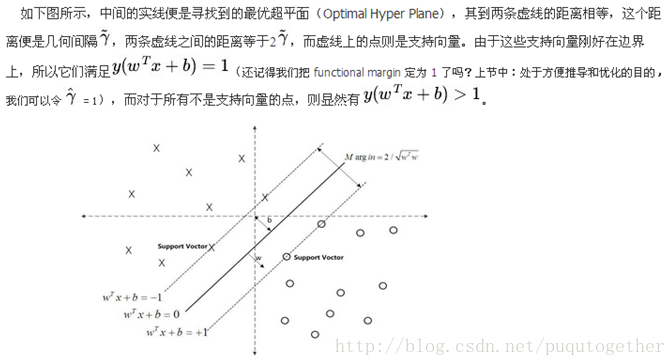
\includegraphics[width=1\textwidth]{fig/hyper.png} % Include the image placeholder.png
\caption{Hyperplane and support vector}
\end{center}
\end{figure}
构造拉格朗日函数求解对偶问题,从而得到原始问题的最优解。
\begin{equation}
\max\limits_{\alpha}\min\limits_{w,b}\mathcal{L}\big(w,b,\alpha \big)= \max\limits_{\alpha}\min\limits_{w,b} \frac{1}{2}\left\|w\right\|^2-\sum_{i=1}^{n}\alpha_i\big( y_i\big(w\cdot x_i+b\big)-1\big)
\end{equation}
通过KKT条件和对偶问题求解(先求极小,导数为0后求解得到w和b的表达式,再代入原式即得对偶问题)由对偶问题可以很容易的引入核函数。
\begin{equation}
\begin{array}{lcl}
\min\limits_{w,b}\mathcal{L}\big(w,b,\alpha \big)= \min\limits_{w,b}\left( \frac{1}{2}\sum\limits_{i,j=1}^{n}\alpha_i\alpha_{j}y_{i}y_{j}x_{i}^{\mathrm{T}}x_j \right. \\ 
\left. -\sum\limits_{i,j=1}^{n}\alpha_i\alpha_{j}y_{i}y_{j}x_{i}^{\mathrm{T}}x_j -b\sum\limits_{i=1}^{n}\alpha_{i}y_i+\sum\limits_{i=1}^{n}\alpha_{i}\right)
\end{array}
\end{equation}
对偶问题优化目标为
\begin{equation}
\begin{array}{lcl}
\min\limits_{\alpha}\quad  \frac{1}{2}\sum\limits_{i,j=1}^{n}\alpha_i\alpha_{j}y_{i}y_{j}x_{i}^{\mathrm{T}}x_j -\sum\limits_{i=1}^{n}\alpha_{i}\\
s.t. \quad \sum\limits_{i=1}^{n}\alpha_{i}y_i=0\\
\quad\quad\quad \alpha_i\ge0,\quad i=1,2,\cdots,n
\end{array}
\end{equation}
解得$\alpha$之后,就可以得到$w$和$b$
\begin{equation}
\begin{array}{lcl}
w^{*}=\sum\limits_{i=1}^{n}\alpha_{i}^{*}y_{i}x_{i}\\
b^*=y_j-\sum\limits_{i=1}^{n}\alpha_{i}^{*}y_{i}\big(x_{i}\cdot x_{j} \big)
\end{array}
\end{equation}
注意这里的下标索引$j$指的是任意一个令$\alpha_j>0$的下标,任取一个,计算出的$b^*$值是相同的。可以观察到,每一个样本都有一个拉格朗日乘子,当样本数增加的时候,需要求解的参数维度太大,很难优化。SMO算法可以降低求解难度。

分离超平面:
\begin{equation}
w^*\cdot x+b^*=0
\end{equation}
分类决策函数
\begin{equation}
f\big(x\big)=\mathrm{sign}\big(w^*\cdot x+b^*\big)
\end{equation}
\end{description} 


\subsection{SMO}
\label{smo}
论文\cite{Platt:Platt1998Sequential},具体推导参考\cite{svm:derivation},推导比李航的书上更详细
 
%----------------------------------------------------------------------------------------
%	SECTION 2
%----------------------------------------------------------------------------------------

\section{算法实现}
见李航书\cite{LiHang:Statistic}
\begin{figure}[H]
\begin{center}
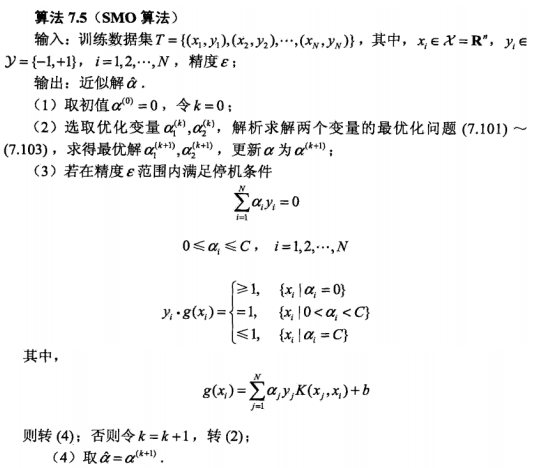
\includegraphics[width=0.8\textwidth]{fig/smo.png} % Include the image placeholder.png
\caption{SMO algorithm}
\end{center}
\end{figure}

实现中的一个小技巧:把$\alpha_2$的索引值搜索范围设置在支持向量索引内,因为非支持向量对应的拉格朗日乘子$\alpha=0$。详细推导见博客\cite{alpha:derive}。

%----------------------------------------------------------------------------------------
%	SECTION 3
%----------------------------------------------------------------------------------------
%
\section{Implementation}
线性核测试
\begin{figure}[H]
\begin{center}
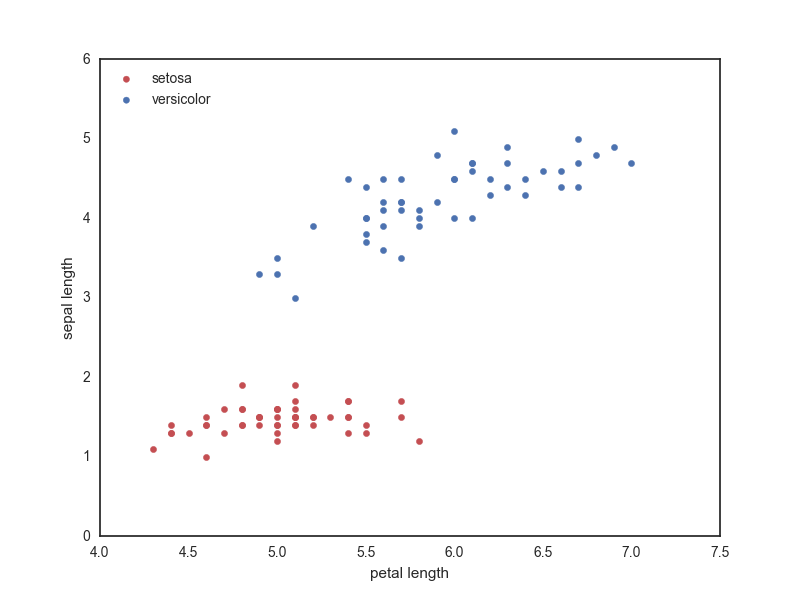
\includegraphics[width=0.8\textwidth]{fig/raw_linear.png} % Include the image placeholder.png
\caption{鸢尾花数据}
\end{center}
\end{figure}

\begin{figure}[H]
\begin{center}
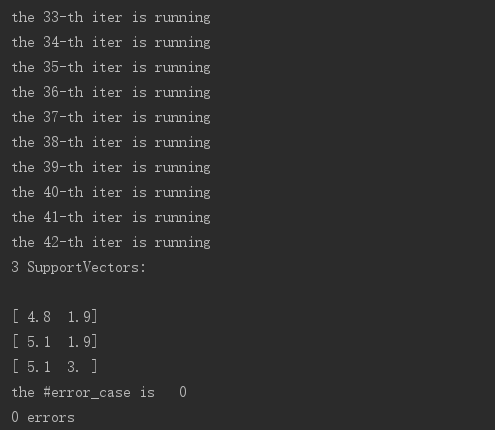
\includegraphics[width=0.8\textwidth]{fig/linear_out.png} % Include the image placeholder.png
\caption{SVM运行结果}
\end{center}
\end{figure}

\begin{figure}[H]
\begin{center}
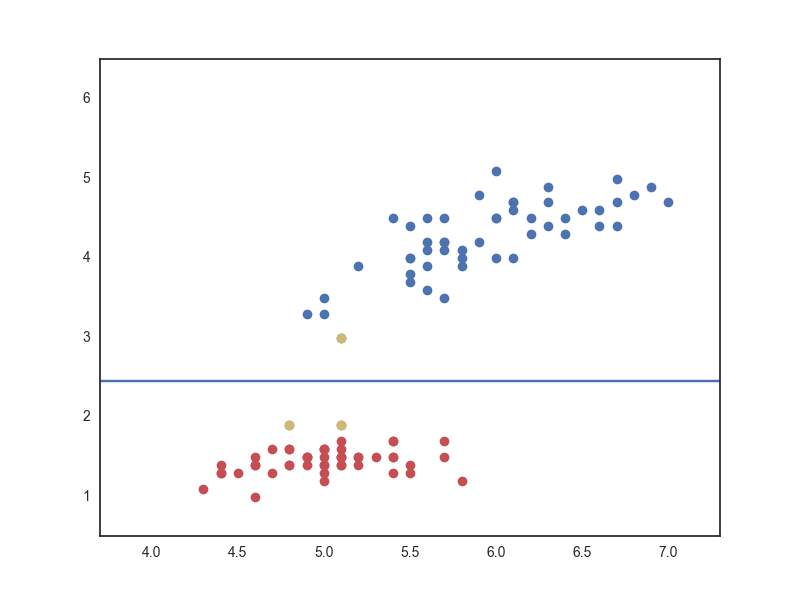
\includegraphics[width=0.8\textwidth]{fig/linear_kernel.png} % Include the image placeholder.png
\caption{SVM分类平面。黄色点为支持向量}
\end{center}
\end{figure}
%\section{Sample Calculation}
%
%\begin{tabular}{ll}
%Mass of magnesium metal & = \SI{8.59}{\gram} - \SI{7.28}{\gram}\\
%& = \SI{1.31}{\gram}\\
%Mass of magnesium oxide & = \SI{9.46}{\gram} - \SI{7.28}{\gram}\\
%& = \SI{2.18}{\gram}\\
%Mass of oxygen & = \SI{2.18}{\gram} - \SI{1.31}{\gram}\\
%& = \SI{0.87}{\gram}
%\end{tabular}
%
%Because of this reaction, the required ratio is the atomic weight of magnesium: \SI{16.00}{\gram} of oxygen as experimental mass of Mg: experimental mass of oxygen or $\frac{x}{1.31}=\frac{16}{0.87}$ from which, $M_{\ce{Mg}} = 16.00 \times \frac{1.31}{0.87} = 24.1 = \SI{24}{\gram\per\mole}$ (to two significant figures).
%
%%----------------------------------------------------------------------------------------
%%	SECTION 4
%%----------------------------------------------------------------------------------------
%
%\section{Results and Conclusions}
%
%The atomic weight of magnesium is concluded to be \SI{24}{\gram\per\mol}, as determined by the stoichiometry of its chemical combination with oxygen. This result is in agreement with the accepted value.
%
%\begin{figure}[h]
%\begin{center}
%\includegraphics[width=0.65\textwidth]{placeholder} % Include the image placeholder.png
%\caption{Partial Gradient of $L_\big(\theta \big)$}
%\end{center}
%\end{figure}
%
%%----------------------------------------------------------------------------------------
%%	SECTION 5
%%----------------------------------------------------------------------------------------
%
%\section{Discussion of Experimental Uncertainty}
%
%The accepted value (periodic table) is \SI{24.3}{\gram\per\mole} \cite{Smith:2012qr}. The percentage discrepancy between the accepted value and the result obtained here is 1.3\%. Because only a single measurement was made, it is not possible to calculate an estimated standard deviation.
%
%The most obvious source of experimental uncertainty is the limited precision of the balance. Other potential sources of experimental uncertainty are: the reaction might not be complete; if not enough time was allowed for total oxidation, less than complete oxidation of the magnesium might have, in part, reacted with nitrogen in the air (incorrect reaction); the magnesium oxide might have absorbed water from the air, and thus weigh ``too much." Because the result obtained is close to the accepted value it is possible that some of these experimental uncertainties have fortuitously cancelled one another.
%
%%----------------------------------------------------------------------------------------
%%	SECTION 6
%%----------------------------------------------------------------------------------------
%
%\section{Answers to Definitions}
%
%\begin{enumerate}
%\begin{item}
%The \emph{atomic weight of an element} is the relative weight of one of its atoms compared to C-12 with a weight of 12.0000000$\ldots$, hydrogen with a weight of 1.008, to oxygen with a weight of 16.00. Atomic weight is also the average weight of all the atoms of that element as they occur in nature.
%\end{item}
%\begin{item}
%The \emph{units of atomic weight} are two-fold, with an identical numerical value. They are g/mole of atoms (or just g/mol) or amu/atom.
%\end{item}
%\begin{item}
%\emph{Percentage discrepancy} between an accepted (literature) value and an experimental value is
%\begin{equation*}
%\frac{\mathrm{experimental\;result} - \mathrm{accepted\;result}}{\mathrm{accepted\;result}}
%\end{equation*}
%\end{item}
%\end{enumerate}

%----------------------------------------------------------------------------------------
%	BIBLIOGRAPHY
%----------------------------------------------------------------------------------------
%
% 注意一定要在文中引用才不会出错(至少引用一个)
\bibliographystyle{plain}
\bibliography{bib//svm}

%----------------------------------------------------------------------------------------


\end{document}